% Template for Cogsci submission with R Markdown

% Stuff changed from original Markdown PLOS Template
\documentclass[10pt, letterpaper]{article}

\usepackage{cogsci}
\usepackage{pslatex}
\usepackage{float}
\usepackage{caption}

% amsmath package, useful for mathematical formulas
\usepackage{amsmath}

% amssymb package, useful for mathematical symbols
\usepackage{amssymb}

% hyperref package, useful for hyperlinks
\usepackage{hyperref}

% graphicx package, useful for including eps and pdf graphics
% include graphics with the command \includegraphics
\usepackage{graphicx}

% Sweave(-like)
\usepackage{fancyvrb}
\DefineVerbatimEnvironment{Sinput}{Verbatim}{fontshape=sl}
\DefineVerbatimEnvironment{Soutput}{Verbatim}{}
\DefineVerbatimEnvironment{Scode}{Verbatim}{fontshape=sl}
\newenvironment{Schunk}{}{}
\DefineVerbatimEnvironment{Code}{Verbatim}{}
\DefineVerbatimEnvironment{CodeInput}{Verbatim}{fontshape=sl}
\DefineVerbatimEnvironment{CodeOutput}{Verbatim}{}
\newenvironment{CodeChunk}{}{}

% cite package, to clean up citations in the main text. Do not remove.
\usepackage{apacite}

% KM added 1/4/18 to allow control of blind submission


\usepackage{color}

% Use doublespacing - comment out for single spacing
%\usepackage{setspace}
%\doublespacing


% % Text layout
% \topmargin 0.0cm
% \oddsidemargin 0.5cm
% \evensidemargin 0.5cm
% \textwidth 16cm
% \textheight 21cm

\title{Combinatorial Capacity of English Negation in Child Language}


\author{{\large \bf Morton Ann Gernsbacher (MAG@Macc.Wisc.Edu)} \\ Department of Psychology, 1202 W. Johnson Street \\ Madison, WI 53706 USA \AND {\large \bf Masoud Jasbi (jasbi@ucdavis.edu)} \\ Department of Linguistics, 469 Kerr Hall, One Shields Avenue \\ Davis, CA 95 USA}


\begin{document}

\maketitle

\begin{abstract}
Negation is very important for langauge and thought. How does it develop
in the language of children? There has been many guessses like
rejection, non-existence, denail, etc. but it has been hard to assess
because these concepts are vaguge. Here we assess the combinatorial
capacity of early negation in children's productions, and use words
negation combines with as a proxy for early concepts expressed by it. We
show some important stuff.

\textbf{Keywords:}
Add your choice of indexing terms or keywords; kindly use a semi-colon;
between each term.
\end{abstract}

\hypertarget{introduction}{%
\section{Introduction}\label{introduction}}

Negation is an abstract concept, lexicalized in all previously studied
human languages, and crucial to everyday communication. It can help a
coffee shop divide its menu into ``coffee'' and ``not coffee'' sections,
with the ``not coffee'' section bringing together diverse items that
otherwise cannot be labeled. It can help us regulate others' actions in
a sign like ``no mask, no entry''. It can also communicate our deepest
wants and dislikes. But how does this crucial abstract concept emerge in
humans? Does language play a role in its emergence or does language
simply adopt it for communication?

There has been several influential hypotheses on the conceptual origin
of negation.

In this paper, we address the same issues with a slightly different
approach. We start with the widely accepted assumption that negation is
a higher order operator or function, operating on lower level concepts.
The question we ask is: what type of concepts does linguistic negation
operate on in early child language? Do we find negation starting in a
limited conceptual domain and then expanding to others? Or do we find it
operating across different conceptual domains as early as we can attest
it?

Darwin (1998) thought that negation has roots in the expression of human
emotions and desires. He hypothesized that the earliest manifestation of
negation and affirmation in infants is when they refuse food from
parents, by withdrawing their heads laterally, or when they accept the
food, by inclining their heads forward. He suggested that head shaking
and nodding as common gestures for negation and affirmation have
developed from this early habit. Considering early functions of negative
morphemes like \emph{no}, many researchers proposed that children use
them to ``reject'' or ``refuse'' (Bloom, 1970; Choi, 1988; Pea, 1978).
For example, they may say ``no'' when asked ``do you want juice?'', say
``not want it'', or say ``don't like it''. Pea (1978) proposed that this
function of negation is the first to emerge in children.

Motor control: prohibition (do not spill milk), inability (I cannot zip
it)

Bloom (1970) suggested that the first function of negation in children's
speech is to express non-existence. Relates to children's development of
object permanence.

Perceptual: non-existence (no juice, no more milk, no fish in the
bathroom, I do not have underpants), failure, Locatives (no in there,
daddy was not on the phone), non-events (the dog not barking)

A third possible domain and path to the acquisition of negation is
language itself. Word learning places its own constraints on the
conceptual space. One possibility is that negation develops, and is
aided by the act of labeling and categorizing objects and actions for
linguistic communication. This function would manifest istelf in
labeling acts with nominal predicates such as ``this is not a bunny'',
``not red'', or ``this isn't a reptile''.

There has been no proposal for negation originating in the child's
understanding of her own or other's epistemic states. In fact, most
development theory of mind accounts assume that this ability emerges
later in children. However, many corpus instances of negation modify
mental state verbs such as \emph{know}, \emph{think}, and
\emph{remember} (e.g.~``I not know''). Therefore, we also report the
prevalence and emergence of such cases.

Caveat on production vs comprehension.

Focusing on the utterance level in this study

\hypertarget{experiments}{%
\section{Experiments}\label{experiments}}

\hypertarget{data-and-preprocessing}{%
\subsection{Data and preprocessing}\label{data-and-preprocessing}}

For developmental data of child language in English, we turned to the
CHILDES database (MacWhinney, 2000), which provides child-parent
conversational
interactions.\footnote{Code and data for our study are in quarantine at https://somewhereonearth.}.
We focused on utterances produced by children with typical development
within the age range of 12 - 72 months, then extracted cases with any of
the three negation markers that are of interest in this study:
\emph{no}, \emph{not} and \emph{n't}. Utterances with only one lexical
token (e.g.~\emph{no !}) were not considered as here we aim to address
particularly the question of what negation markers could \emph{combine}
with. Preprocessing led to a data set of 365,260 utterances with
negation structures from a total of 811 children across 56 corpora.

Figure @ref(fig:speaker\_stats)

\begin{CodeChunk}
\begin{figure}[H]

{\centering 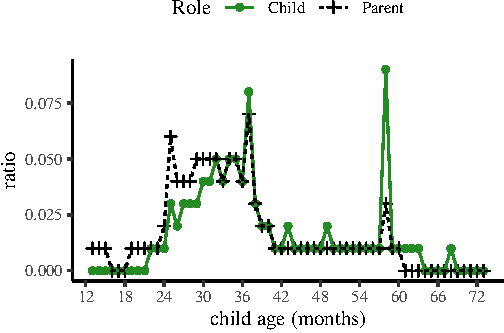
\includegraphics{figs/speaker_stats-1} 

}

\caption[Distribution of the number of utterances with negative morphemes in child and parent speech]{Distribution of the number of utterances with negative morphemes in child and parent speech.}\label{fig:speaker_stats}
\end{figure}
\end{CodeChunk}

\hypertarget{negation-domains}{%
\subsection{Negation domains}\label{negation-domains}}

In this section, we describe in details our automatic extraction of
syntactic structures that express different types of negation concepts.
The current English data from CHILDES contains morphosyntactic
information (Sagae, Davis, Lavie, MacWhinney, \& Wintner, 2010) such as
part-of-speech (POS) information as well as grammatical or syntactic
dependency
relations.\footnote{Besides using the provided POS and syntactic dependency information in CHILDES, we also experimented with the state-of-the art parser from Stanza [@qi-etal-2020-stanza]. There were no worth noting differences in the analyses for the negation constructions.}
We take advantage of information as such when automatically identifying
our constructions of interest. An utterance with negative morpheme(s)
was only considered when the negative morphemes has either a POS of
\emph{neg} or \emph{qn}, the latter of which was mainly for cases with
\emph{no} as a quantifier. Furthermore, the syntactic functions and
relations of the negative morphemes should not be enumeration (\emph{no
no no}), communicators or discourse markers

After extracting all instances with negative morphemes, the
developmental trajectory of each construction type as described in the
previous section was analyzed. While the matter of interest here is
child speech, we also compared patterns in child production to those in
parent speech as references at the corresponding age of the child. Then
we combined the development of all construction types for analysis as a
whole

\hypertarget{emotion}{%
\subsubsection{Emotion}\label{emotion}}

In order to investigate utterances that express emotions, particularly
the concept of rejections, we focused on specific cases where the lemma
form of the head verb of the phrase is either \emph{like} or
\emph{want}, and the head verb is modified by one of the three negative
morphemes. Each of the utterances either takes a subject or has no
subject at all. And the existence of a subject was determined via
searching for a word in the utterance that has the \emph{SUBJ}
dependency relation with the head verb.

Additionally, other than expressions that the speaker used to describe
their own emotions (e.g.~(1)) or their (in)ability to do so, we also
included cases that express rhetorical inquiries of emotions from one
interlocutor addressed to another (e.g.~(3)) as well as instances where
the speaker is describing the emotions of somebody else (e.g.~(4)).
Overall our data extraction resulted in a total of 21,034 utterances
(Child: 9,608; Parent: 11,426).

~ (1) \emph{I no like sea} / \emph{don't wanna go} ~ (2) \emph{I can't
like that} ~ (3) \emph{don't you wanna try it} ~ (4) \emph{Sarah doesn't
like that either} ~

To compare the patterns between child and parent speech, for each
domain, we calculated the relative ratio of (i) each of the three
negative morphemes overall; (ii) usage of negative morphemes with the
two different head verbs; (iii) utterances expression emotion with the
three negative morphemes at different ages of the child. In both child
and parent speech, when expressing emotion with either of the two head
verbs \emph{like} and \emph{want}, the most frequently used negative
morpheme is \emph{n't} combined with an auxiliary verb. Comparing the
two different head verbs, overall the negative morphemes are co-occur
with \emph{want} more frequently.

On the other hand, when looking at the developmental trajectory, as
presented in Figure @ref\{fig:emotion\}, children's usage of negative
morphemes is comparable regardless of the particular head verb. In
general, children did not start using negative morphemes in this domain
until the age of 7 months; their usage of these morphemes for the
concept of rejection is the most frequent during the age range of 13 -
21 months, then gradualy decreases as they age.

\begin{CodeChunk}
\begin{figure}[H]

{\centering 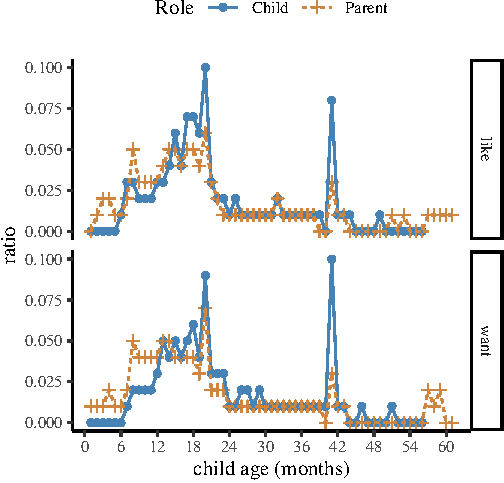
\includegraphics{figs/emotion-1} 

}

\caption[Emotion]{Emotion}\label{fig:emotion}
\end{figure}
\end{CodeChunk}

\hypertarget{theory-of-mind}{%
\subsubsection{Theory of mind}\label{theory-of-mind}}

With regards to the domain of theory of mind, we attended to cases that
express epistemic position. Specifically, we focused on utterances that
articulate the concept of unknowing (e.g.~(5)) or uncertainty
(e.g.~(6)). The cases that were subject to analyses here included either
\emph{know}, \emph{remember} or \emph{think} as the head verb, modified
by the negative morphemes or the combination of the negative morphemes
with auxiliaries. By these search criteria, instances where the speaker
inquires about or describes the epistemic position of another speaker
(e.g.~(7)) were also selected. This led to a subset of 32,793 utterances
in total (Child: 10,389; Parent: 22,404).

~ (5) \emph{I not know} / \emph{I didn't remember} (6) \emph{I don't
think so} (7) \emph{don't you remember} / \emph{She doesn't know this} ~

In both child and parent speech, the most frequently used negative
morpheme in expressing epistemic position is \emph{n't}, a pattern that
is consistent across the three different head verbs. And the negative
morphemes tend to co-occur more often in cases that describes the state
of unknowing, which is indicated mainly by the verb \emph{know}. Given
results from Figure @ref\{fig:epistemic\}, there does not seem to be a
quite consistent developmental trajectory of child speech in the domain
of theory of mind. While regardless of the head verb, children appeared
to start applying the negative morphemes in this domain around the age
of 4. Nevertheless, there seems to be more variability in expressing an
epistemic position with \emph{remember} and \emph{think} as the children
age. By contrast, the pattern for instances with \emph{know} gradually
decreases after the age of 16 months.

\begin{CodeChunk}
\begin{figure}[H]

{\centering 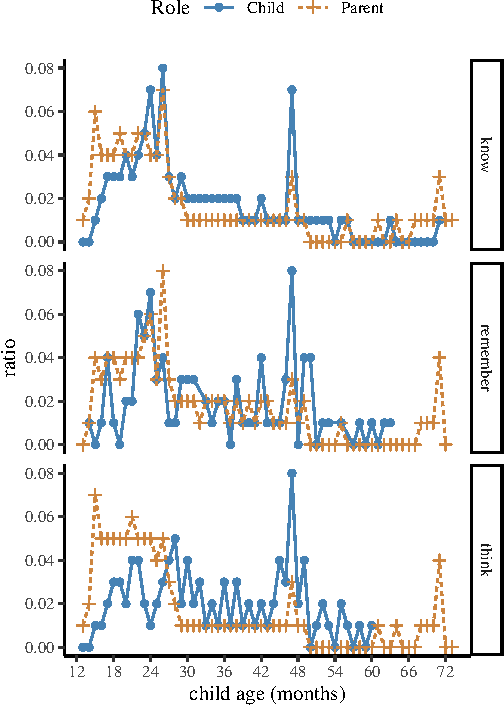
\includegraphics{figs/epistemic-1} 

}

\caption[Theory of mind]{Theory of mind}\label{fig:epistemic}
\end{figure}
\end{CodeChunk}

\hypertarget{motor-control}{%
\subsubsection{Motor control}\label{motor-control}}

For utterances that articulate the concept of motor control, we focused
on two individual aspects with different communicative functions. The
first one includes cases that indicate prohibition (e.g.~(8)), and the
second one contain cases that articulate inability (e.g.~(9)). For the
former, we analyzed cases where the negative morphemes are combined with
the auxiliary verb \emph{do} (\emph{do}, \emph{does}, \emph{did}) and
the auxiliary does not take any subject; whereas for the latter, we
analyzed cases where the negative morphemes co-occur with the auxiliary
\emph{can} (\emph{can} and \emph{could}). For both functions, the
negative morphemes and the auxiliary together modifies a head verb. In
order to not overlap with the domain of Emotion, Theory of Mind and
Perception (see below), our search excluded cases where the head verb
has any of the following lemma forms: \emph{like}, \emph{want},
\emph{know}, \emph{think}, \emph{remember}, \emph{have}.

For inability in particular, cases that do not have a subject
(\emph{can't play}) or contain a subject other than I (\emph{you can't
do that}) could yield ambiguous readings without taking a larger
discourse context into account; they could be a rhetorical question or
also express the concept of prohibition. Therefore to avoid potential
ambiguity, we excluded instances as such. In other words, when searching
for utterances that articulate inability, we restricted our analyses
only to cases with a subject \emph{I}. This led to a subset of 235
utterances (Child: 113; Parent: 122).

~ (8) \emph{do}: \emph{don't blame Charlotte}

~ (9) \emph{can}: \emph{I can't see}

Again for comparison of child and parent speech, we calculated the
relative ratio of (i) each of the three negative morphemes overall; (ii)
usage of negative morphemes with the two different communicative
functions; (iii) utterances expression motor control with the three
negative morphemes at different ages of the child. Overall the most
frequently used negative morpheme is \emph{n't} when applied in the
domain of motor control. Comparing the two communicative functions, the
negative morphemes tend to co-occur more often when expressing
inability.

As shown in Figure @ref\{fig:motor\_control\}, the developmental
trajectory of using the negative morphemes in the domain of motor
control is similar to that in the domain of emotion. Children started
combining negative morphemes in syntactic structures that epxress
prohibiiton and inability around the age of 6 months, then gradually
increases until the age of 22 months.

\begin{CodeChunk}
\begin{figure}[H]

{\centering 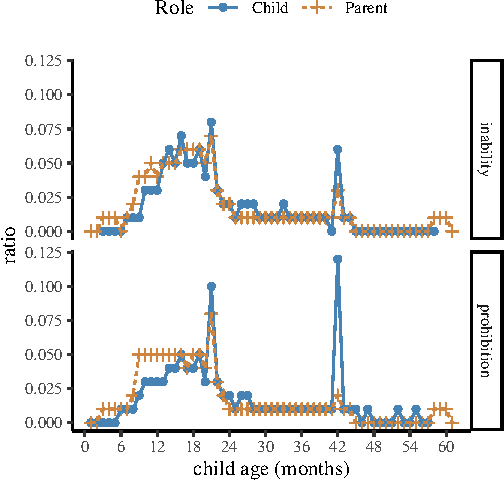
\includegraphics{figs/motor_control-1} 

}

\caption[Motor control]{Motor control}\label{fig:motor_control}
\end{figure}
\end{CodeChunk}

\hypertarget{language-learning}{%
\subsubsection{Language learning}\label{language-learning}}

Within the domain of language learning, we concentrated on cases where
negative morphemes are adopted to label the identity (e.g.~(10)), and/or
characteristics (e.g.~(11)) of a predicative nominal. In addition, we
also included instances where the negators are used to modify a
predicative adjective (e.g.~(12)). Following these criteria, utterances
where the negative morpheme is modifying a nominal or adjectival
predicate of a copula verb were extracted. None of the utterances
contain expletives (\emph{there is no book}). The existence of a
predicate was identified with the help of POS information and dependency
relation. The POS of the predicate has to be either noun (\emph{n}) or
adjective (\emph{adj}), and its dependency relation with the copula has
to be \emph{PRED}. This resulted in a total of 27,689 utterances (Child:
55 utterances; Parent: 61 utterances).

~ (10) \emph{that's not a farmer} (11) \emph{I'm not a heavy baby Mum}
(12) \emph{It's no good} ~

Again for comparison of child and parent speech, we calculated the
relative ratio of (i) each of the three negative morphemes overall; (ii)
usage of negative morphemes with the two different communicative
functions; (iii) utterances expression motor control with the three
negative morphemes at different ages of the child. Overall the most
frequently used negative morpheme is \emph{n't} when applied in the
domain of motor control. Comparing the two communicative functions, the
negative morphemes tend to co-occur more often when expressing
inability.

Comparing the three negative morphemes, the most frequently used is
\emph{not} in both child and parent speech. Based on results from Figure
@ref\{fig:learning\}, the developmental trajectory of using the negative
morphemes in the domain of language learning is comparable to previous
domains. Children started using the negative morphemes for the function
of labeling nominal objects around the age of 7 months and their usage
as such became more regular around the age of 10 months. However, the
frequency of applying the negative morphemes in the language learning
domain began to decrease around the age of 18 months.

\begin{CodeChunk}
\begin{figure}[H]

{\centering 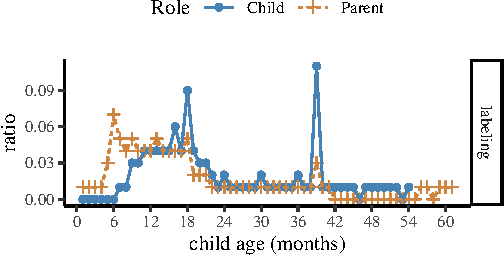
\includegraphics{figs/learning-1} 

}

\caption[Language learning]{Language learning}\label{fig:learning}
\end{figure}
\end{CodeChunk}

\hypertarget{perception}{%
\subsubsection{Perception}\label{perception}}

The last domain to be analyzed here is Perception, with two particular
functions. First one is indication of non-existence, while the second
one denotes possession. For expressions of non-existence, we extracted
utterances that either have expletives marked by \emph{there}
(e.g.~(13)), or cases where the negative morphemes are modifying a
nominal (i.e.~its syntactic head based on the CHILDES annotation is a
nominal; e.g.~(14)). For expressions of possession, we selected
utterances where the negative morphemes are modifying a possessive
pronoun, as well as instances where the negative morphemes are combined
with auxiliary verbs to modify a head verb with the lemma form
\emph{have} (e.g.~(15)). With utterances such (14) and (15), in order to
not confuse with the domain of Language Learning, we did not include any
cases where the syntactic head of the negative morphemes is a predicate
of a copula verb. As a result, our search did not find any utterances
that express the function of possession in this case, and the total of
utterances that were subjected to analysis in this domain is 23,408
(Child: 55; Parent: 61). (13) \emph{there's no water} (14) \emph{no
(more) candy} / \emph{not in your mouth} (15) \emph{not mine} / \emph{I
don't have it}

In both child and parent speech, the most frequently occurred negative
morphemes in the domain of Perception is \emph{no}. Again for comparison
of child and parent speech, we calculated the relative ratio of (i) each
of the three negative morphemes overall; (ii) usage of negative
morphemes with the two different communicative functions; (iii)
utterances expression motor control with the three negative morphemes at
different ages of the child. Overall the most frequently used negative
morpheme is \emph{n't} when applied in the domain of motor control.
Comparing the two communicative functions, the negative morphemes tend
to co-occur more often when expressing inability.

As shown in Figure @ref\{fig:perception\}, the developmental trajectory
of using the negative morphemes in the domain of Perception is also
comparable to previous domains. Children began applying the negative
morphemes to this domain around the age of 8 months and their usage
gradually increased after the age of 11 months. Similarly to the domain
of Language Learning, the frequency of using the negative morphemes in
indicating non-existence started to decrease around the age of 19
months.

\begin{CodeChunk}
\begin{figure}[H]

{\centering 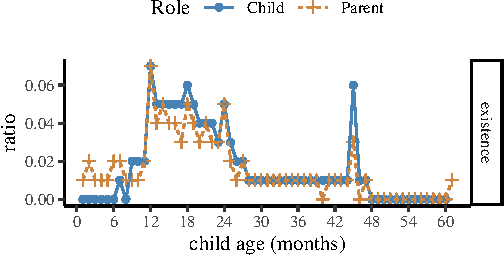
\includegraphics{figs/perception-1} 

}

\caption[Perception]{Perception}\label{fig:perception}
\end{figure}
\end{CodeChunk}

\hypertarget{an-overall-look-at-all-domains}{%
\subsubsection{An overall look at all
domains}\label{an-overall-look-at-all-domains}}

\begin{figure*}[h]
\begin{CodeChunk}
\begin{figure}[H]

{\centering 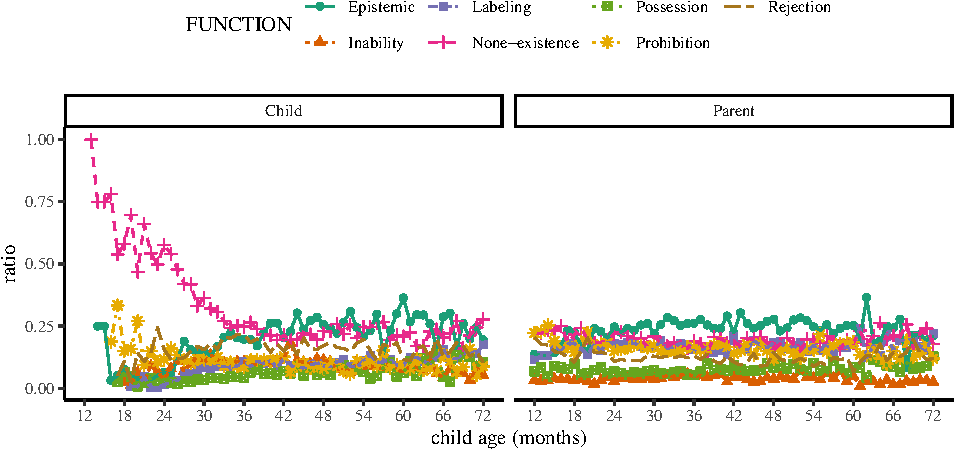
\includegraphics{figs/all-1} 

}

\caption[All domains]{All domains}\label{fig:all}
\end{figure}
\end{CodeChunk}
\end{figure*}

\hypertarget{discussion}{%
\section{Discussion}\label{discussion}}

\hypertarget{references}{%
\section{References}\label{references}}

\setlength{\parindent}{-0.1in} 
\setlength{\leftskip}{0.125in}

\noindent

\hypertarget{refs}{}
\leavevmode\hypertarget{ref-bloom1970language}{}%
Bloom, L. M. (1970). \emph{Language development: Form and function in
emerging grammars} (PhD thesis). Columbia University.

\leavevmode\hypertarget{ref-choi1988semantic}{}%
Choi, S. (1988). The semantic development of negation: A
cross-linguistic longitudinal study. \emph{Journal of Child Language},
\emph{15}(3), 517--531.

\leavevmode\hypertarget{ref-darwin1872expression}{}%
Darwin, C. (1998). \emph{The expression of the emotions in man and
animals}. John Murray.

\leavevmode\hypertarget{ref-macwhinney2000childes}{}%
MacWhinney, B. (2000). \emph{The childes project: Tools for analyzing
talk. Transcription format and programs} (Vol. 1). Psychology Press.

\leavevmode\hypertarget{ref-pea1978}{}%
Pea, R. (1978). \emph{The development of negation in early child
language} (PhD thesis). University of Oxford.

\leavevmode\hypertarget{ref-sagae2010morphosyntactic}{}%
Sagae, K., Davis, E., Lavie, A., MacWhinney, B., \& Wintner, S. (2010).
Morphosyntactic annotation of childes transcripts. \emph{Journal of
Child Language}, \emph{37}(3), 705--729.

\bibliographystyle{apacite}


\end{document}
